\section{Method}
% incurs a substantial time cost to search for an optimal planning route.
\begin{figure*}

    \centering
    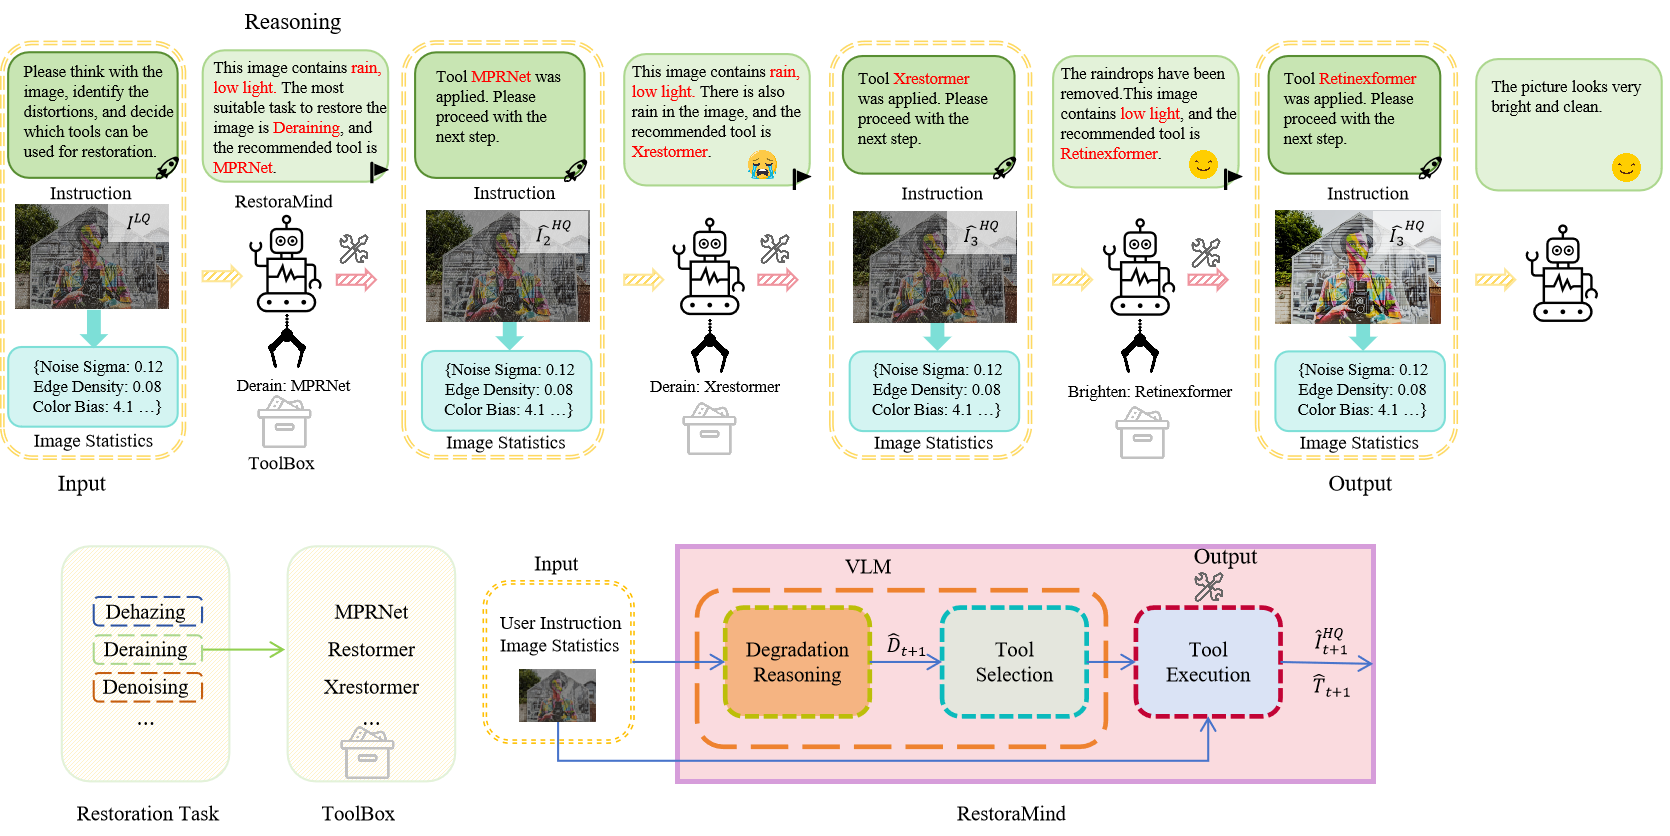
\includegraphics[width=0.9\linewidth]{sec/fig/fig2.png}
    \caption{\textbf{Overview of RestoraMind.} The agent utilizes a Vision-Language Model (VLM) to perceive the degraded image and its statistical priors.It operates in a loop of \textbf{Degradation Reasoning}, \textbf{Tool Selection}, and \textbf{Tool Execution}.By treating restoration as a sequential decision-making task, RestoraMind dynamically selects the most appropriate expert tool from the toolbox at each step to iteratively recover the high-quality image $\hat{I}^{HQ}$.}
    \label{fig:pipeline}
\end{figure*}



% Our method recasts the problem of real-world image restoration as a sequential decision-making process. We introduce an agent named \textbf{Restoramind}, which has a powerful Vision-Language Model at its core. Unlike AiOIR models that attempt to predict all degradations at once or follow a fixed restoration pipeline, Restoramind is trained via Reinforcement Learning to dynamically interact with the restoration environment.

% The core innovation of Restoramind lies in its \textbf{Tool-Interactive Reasoning}. At each time step, the agent first perceives the current state of the image, then plans and executes an action—selecting a restoration tool from a specialized toolbox. Most critically, it observes the resulting image after the tool is applied and reflects on the consequences of this action, thereby enhancing its understanding of both the image state and the tool's efficacy.


\subsection{Overview}
\noindent
RestoraMind aims to recover a high-quality image $\hat{I}^{HQ}$ from a degraded observation $I^{LQ}$, which has undergone an unknown and complex degradation process $D$. The process $D$ typically consists of multiple degradation types $\{D_1, D_2, \dots, D_n\}$, such as haze, noise, and defocus blur. 
Instead of handling all degradations at once, RestoraMind formulates image restoration as a \textbf{sequential decision-making process}, where it iteratively reasons about the remaining degradation types in the current image and selects the suitable restoration tool from $\mathcal{A}$ based its low-level statistics for restoration. The final tool execution order, intermediate restored results and the predicted degrdatation types are denoted as $\hat{T} = \{\hat{T}_1, \hat{T}_2, \dots, \hat{T}_n\}$ and $\hat{I}^{HQ} = \{\hat{I}_1^{HQ}, \hat{I}_2^{HQ}, \dots, \hat{I}^{HQ}\}$, and ${\hat{D} = \{\hat{D}_1, \hat{D}_2, \dots, \hat{D}_n\}}$, respectively.
Taking step $S_t$ as example, RestoraMind receives the previously restored image $\hat{I}^{HQ}_{t-1}$, its low-level image statistics, an instruction prompt describing the tools used so far $\{\hat{T}_1, \dots, \hat{T}_{t-1}\}$, and contextual information such as the image description and restoration goal. 
It first predicts the remaining degradations and then selects the appropriate tool to restore the current image. 
The newly restored result $\hat{I}^{HQ}_{t}$ and the updated tool history $\{\hat{T}_1, \dots, \hat{T}_{t}\}$ are propagated to the next state. \textbf{Owing to its capabilities in both degradation perception and tool utilization}, RestoraMind efficiently restore complex and unknown degradations in near-linear time with respect to the number of degradation types, without requiring explicit rollback or brute-force search strategies, as illustrated in Fig.~\ref{fig:pilot_study} (c).


% \subsection{Agentic Reinforcement Learning}
% \noindent\textbf{Training policy.}
% RestoraMind build upon the Q-insight, a visual perception VLLMs for image quality assessment as the cold start. It is trained via a end-to-end reinforcement learning, aims to master both capability of degradation reasoning and tool using. The overview of the training policy are illustrated in Fig.~\ref{fig.overview}. At each step, the RestoraMind is imposed to first reason the degradtion types and then daptitively select a tool for restore the current image. The state transintion is do


% \noindent\textbf{Tool selection within the same degradation types.}

% \noindent\textbf{Reward function.}

% \section{Method}
% \label{sec:method}
\subsection{Agentic Reinforcement Learning}
% We initialize RestoraMind with \emph{Q-insight}, a degradation-aware VLLM pretrained for perceptual quality assessment. We train RestoraMind within an end-to-end reinforcement learning framework, enabling it to jointly master degradation reasoning and tool utilization. The overall training pipeline is illustrated in Fig.~\ref{}. 
\noindent\textbf{Training pipeline.}
We initialize RestoraMind with \emph{Q-insight} \cite{li2025q}, a degradation-aware VLLM pretrained for perceptual quality assessment. We train RestoraMind within an end-to-end reinforcement learning framework~\cite{sheng2025hybridflow}, enabling it to jointly master degradation reasoning and tool utilization. The overall training pipeline is illustrated in Fig.~\ref{fig:pipeline}. At each state, the agent first predicts the degradation types of the distorted image and then adaptively selects one restoration tool from the toolbox for restoration. The predicted degradation types, the restored image, and the selected tool form a triplet that serves as the input for the next state, where the restored image serving as the new observation. In subsequent states, the agent further reasons about the remaining degradation types and assesses whether the tool used in the previous step has removed the corresponding degradation. When the degradation remains, the agent rolls back to the previous state and re-restores the original image or previous observation using an alternative tool of the same degradation type. The agent switches to tools handling other degradation types once the previous degradation has been either resolved or remains after the reprocessing attempt. When the agent fails to restore all degradations within a fixed number of dialogue rounds, it receives a low reward, encouraging exploration of more effective tool execution sequences in future iterations. Policy parameters are updated from on-policy rollouts using a standard policy-gradient (PPO) ~\cite{schulman2017proximal} with generalized advantage estimation and an entropy regularizer to sustain exploration. 

% At step $S_t$, the agent first predicts the remaining degradation types $\hat{D}_t=\{\hat{D}_1,\hat{D}_2,\dots\}$ and then selects a tool $\hat{T}_t\in\mathcal{A}$ that is most suitable for the current image. Executing $\hat{T}_t$ yields the updated result $\hat{I}^{HQ}_{t}$, which—together with the updated history $\{\hat{T}_1,\dots,\hat{T}_t\}$—is passed to the next step $S_{t+1}$ for re-analysis. The episode terminates when the confidence that all degradations have been removed exceeds a preset threshold or when a small step budget $T_{\max}$ is reached. We optimize the policy with a standard policy-gradient algorithm (e.g., PPO) using the shaped reward described in Sec.~\ref{sec:reward}. During early training, we apply action masking to suppress tools inconsistent with the current $\hat{D}_t$ and gradually relax this mask to encourage exploration. This design avoids planning a full tool sequence in advance: the agent commits only to the next action based on the presently observed artifacts, and can retry a different tool within the same degradation type or switch to another type when the evidence supports it (see Sec.~\ref{sec:intra-type} and Fig.~\ref{fig:overview}).
\noindent\textbf{Adaptive tool selection within the same degradation type.}
A single degradation type often corresponds to multiple expert tools, each designed with distinct architectures and training strategies. This raises an key question: \textit{does a universally superior model exist that performs consistently well across all images within the same degradation domain?} To explore this, we conduct a pilot study (Fig.~\ref{fig:pilot_study}) by applying three degradation types, \textit{i.e.}, noise, blur, and rain, to two different images and restoring them with their corresponding expert models. The results reveal the complementarity between tools handling the same degradation type. This observation motivates us to not only optimize the execution order of tools but also to enable the agent to reason about tool selection within the same degradation domain. Previous methods~\cite{zhu2024intelligent,zuo20254kagent,chen2024restoreagent} typically rely on textual descriptions collected from GitHub or HuggingFace to help the model understand the functionality of each tool. However, such high-level descriptions are detached from the visual content and lack explicit cues about low-level image priors. To bridge this gap, we compute a set of lightweight image statistics such as color distribution, contrast, edge density, and brightness using traditional image processing techniques. These statistics can be obtained with negligible computational cost and are organized into a structured format that is fed into the agent at each decision state. This design allows the agent to leverage image-specific characteristics when selecting the suitable restoration tool for the current degraded input.

% Image priors such as color, contrast, edge density, and brightness can be efficiently computed through traditional image processing techniques. Building upon this, we extract a set of statistical image features from multiple perspectives and incorporate them into the agent’s decision process, allowing it to select the most suitable restoration tool tailored to the specific image distribution.

% Many degradation types have multiple complementary tools. Instead of hard-coding a fixed mapping, RestoraMind learns an \emph{intra-type} selector. When the top predicted type is $d$, we restrict candidates to $\mathcal{A}_d=\{a^{(d)}_1,\dots,a^{(d)}_m\}$. The agent forms a compact context vector
% \[
% z_t=\mathrm{Enc}(I_t)\,\oplus\,\phi(\hat{p}_t)\,\oplus\,\psi(a_{t-1}),
% \]
% where $\mathrm{Enc}(\cdot)$ extracts lightweight image statistics and VLLM features, $\phi(\cdot)$ embeds the remaining-degradation distribution, and $\psi(\cdot)$ encodes the previous action. Each candidate tool has an embedding $e(a)$. The intra-type logits are
% \[
% q(a\mid d,s_t)=\mathrm{MLP}\!\big(z_t\oplus e(a)\big), \quad a\in\mathcal{A}_d,
% \]
% and the policy samples from $\mathrm{softmax}(q)$. To improve robustness, we include a \emph{retry gate}: if the post-tool re-analysis indicates that type $d$ persists, the agent is allowed a small number of retries with a \emph{different} tool in $\mathcal{A}_d$ before switching types. We further add a dueling preference term that, when two tools from the same type are tried in similar contexts and lead to different downstream returns, encourages the higher-return tool to have a larger logit margin.
\noindent\textbf{Reward function.}
At step $t$, the agent receives a shaped reward defined as
\begin{equation}
\label{eq:reward_total_main}
r_t=\alpha\,\Delta Q_t+\beta\,R_{\text{deg}}(\hat{\mathcal D}_t,\mathcal D)-\gamma\,\mathrm{Cost}(a_t)-\delta,
\end{equation}
where $\Delta Q_t = R_{\text{quality}}(I_{t+1})-R_{\text{quality}}(I_t)$ measures the perceptual improvement of the restored image, and $R_{\text{deg}}$ quantifies the correctness of degradation reasoning.

\vspace{3pt}
\noindent\textit{Quality reward.}
The composite quality score is formulated as
\[
\begin{aligned}
R_{\text{quality}}(I) =\;
&\lambda_{\text{psnr}}\,\mathrm{PSNR}_{\text{norm}}(I,I_{HQ}) \\
&+\lambda_{\text{ssim}}\,\mathrm{SSIM}_{\text{norm}}(I,I_{HQ}) \\
&+\lambda_{\text{lpips}}\big(1-\mathrm{LPIPS}_{\text{norm}}(I,I_{HQ})\big),
\end{aligned}
\]

which integrates normalized PSNR, SSIM, and LPIPS metrics, each scaled to the range [0,1] through affine normalization.
The normalization weights $\lambda_{\text{psnr}}$, $\lambda_{\text{ssim}}$, and $\lambda_{\text{lpips}}$ are detailed in the supplementary material.

\vspace{3pt}
\noindent\textit{Reasoning reward.}
For reasoning accuracy, let $\hat{\mathcal D}_t$ denote the set of predicted degradation types at step $t$, and $\mathcal D$ the ground-truth set (available for synthetic training data).
We define
\[
R_{\text{deg}}(\hat{\mathcal D}_t,\mathcal D)=
\frac{\lvert \hat{\mathcal D}_t\cap \mathcal D\rvert}{\max(1,\lvert \hat{\mathcal D}_t\rvert)},
\]
which measures the proportion of correctly identified degradation types.
When ground-truth annotations are unavailable (e.g., real-world images), this term is omitted or replaced with a self-consistency proxy.

\vspace{3pt}
\noindent\textit{Efficiency penalty.}
The $\mathrm{Cost}(a_t)$ term penalizes latency or resource-intensive tools, while $\delta$ introduces a small per-step penalty to encourage concise restoration sequences.
Upon termination, a terminal reward
$r_{\text{final}}=\kappa\,R_{\text{quality}}(I_T)$
or a failure penalty is assigned, aligning the learning objective with achieving high-quality restoration using minimal steps.


% \paragraph{Practical Training Details.}
% We train with PPO and generalized advantage estimation, an entropy bonus for exploration, and mixed rollouts: (i) real images with unknown ground truth (reward from $R_{\text{quality}}$ and no-reference signals in Q-insight) and (ii) synthetic multi-degradation data with reference supervision for $R_{\text{quality}}$ and $R_{\text{deg}}$. Action masking is annealed during training; a per-type minimum exploration rate prevents collapse to a single favored tool. We maintain a small replay buffer of difficult contexts (where $\Delta Q_t$ stagnates) to refresh failure modes. Unless stated otherwise, termination uses a fixed $T_{\max}$ and a confidence threshold on the remaining-degradation mass inferred from $\hat{p}_t$.





% \subsection{Core Components of Restoramind}
% \subsubsection{VLM as the Reasoning Core}
% We utilize Q-Insight as the core of \textbf{Restoramind}. Li et al. employed Reinforcement Learning (GRPO, Group Relative Policy Optimization) to elicit and constrain the model's visual reasoning capabilities, achieving quality score regression and degradation perception. Building on this foundation, we further stimulate its degradation perception capabilities by using RL on a dataset comprising various combinations of degradation types. Subsequently, it undergoes RL training for interactive image restoration within the tool-based environment. This methodology preserves the VLM's inherent complex language reasoning capabilities while simultaneously endowing it with robust visual degradation perception. This dual capability enables the agent to transition from mere artifact detection to a deeper comprehension of their complex interrelationships and spatial characteristics. For instance, it can formulate a sophisticated plan by reasoning that, "motion blur is localized at the image edges, whereas noise is more significant in smooth areas, thus denoising should be a prioritized first step."

% \subsubsection{The Modular Restoration Toolbox}
% The agent's action space is defined by a restoration toolbox $\mathcal{A}$. We do not adopt an All-in-One model because such models often sacrifice task-specific performance when handling multiple tasks and struggle to generalize to unseen degradations. Instead, we employ a collection of expert models, as these specialized tools typically provide superior performance on their respective sub-tasks. Our toolbox contains $N$ pre-trained restoration networks, such as a denoising tool, a deblurring tool, etc.

% \subsubsection{Reinforcement Learning Formulation for Interactive Restoration}
% To train the agent via Reinforcement Learning, we formalize the decision-making process as a Markov Decision Process (MDP), defined by a tuple $(S, A, P, R)$:

% \paragraph{State Space}
% At time step $t$, the agent must perceive the current image and the history of operations. Therefore, we define the state as $s_t = (I_t, h_t)$, where $I_t$ is the image tensor at the current time step, and $h_t$ is a text string describing the sequence of actions executed from the initial state to the present. A single image $I_t$ fails to capture the full Markovian state, as visually similar images may arise from distinct restoration paths—a phenomenon known as perceptual aliasing. The inclusion of the history $h_t$ is therefore essential, augmenting the visual percept with the necessary contextual trajectory to disambiguate the state and enable effective, non-myopic planning.

% \paragraph{Action Space}
% The action space is a discrete set comprising all tools in the toolbox plus a stop action, i.e., $A = \{\tau_1, \tau_2, \ldots, \tau_N, \tau_{\text{stop}}\}$.

% \paragraph{State Transition}
% In our framework, the state transition is deterministic, as the application of a tool is a deterministic function. When the agent executes an action $a_t$ (i.e., selecting tool $\mathcal{T}_i$) in state $s_t = (I_t, h_t)$, the next state $s_{t+1} = (I_{t+1}, h_{t+1})$ is uniquely determined. This transition is manifested in two ways: first, the current image $I_t$ transitions to the new state $I_{t+1}$ via the tool invocation. Second, the contextual state is updated by appending the currently executed action $a_t$ to $h_t$, yielding the new history sequence $h_{t+1} = \{a_0, \ldots, a_{t-1}, a_t\}$.

% This deterministic state transition is the cornerstone of our "interactive restoration" paradigm. It guarantees that the subsequent state $s_{t+1}$ presented to the agent encapsulates the exact visual consequence, $I_{t+1}$, of its immediately preceding action $a_t$. This structural design compels the VLM to establish a direct causal link between its intended plan and the resulting perceptual feedback. It is this explicit, closed-loop mechanism that underpins the agent's capacity for reflective reasoning and iterative policy refinement.


% \paragraph{Reward Function}
% A crucial component of the reward function is the measure of image quality, which is essential for driving the agent's learning. We use full-reference metrics to calculate an image quality reward $R_{\text{quality}}(I)$, which combines PSNR, SSIM, and LPIPS:
% $$
% \begin{aligned}
% R_{\text{quality}}(I) &= \lambda_{\text{psnr}}\text{PSNR}_{\text{norm}}(I, I_{HQ}) \\
% &+ \lambda_{\text{ssim}}\text{SSIM}_{\text{norm}}(I, I_{HQ}) \\
% &+ \lambda_{\text{lpips}}(1 - \text{LPIPS}_{\text{norm}}(I, I_{HQ}))
% \end{aligned}
% $$
% To ensure these metrics contribute on a comparable scale, we normalize them to the [0, 1] range:
% \begin{align}
%     \text{PSNR}_{\text{norm}} &= \sqrt{\max\left(0, \min\left(1, \frac{\text{PSNR} - 10}{30}\right)\right)} \\
%     \text{SSIM}_{\text{norm}} &= \frac{\text{SSIM} + 1}{2} \\
%     \text{LPIPS}_{\text{norm}} &= \max(0, \min(1, \text{LPIPS}))
% \end{align}

% \subsection{RestoraMind: Composite Reward Optimization with GRPO}
% \subsubsection{Policy Optimization with GRPO}
% For a policy network with complex reasoning and generation capabilities like a VLM, standard policy gradient methods can face challenges in exploration and convergence. Therefore, we employ GRPO for optimization. GRPO is an innovative RL paradigm that significantly reduces the computational burden by calculating advantages through the comparison of a group of responses sampled from the policy model. Specifically, at each state $s_t$, we sample a group of $G$ candidate actions $\{a_t^i\}_{i=1}^G$ from the current policy $\pi_{\theta_{old}}$. For each candidate action $a_t^i$, we execute it to obtain a reward $r_i$. The core idea of GRPO is to compute the group-relative advantage $A_i$ for each candidate action $a_t^i$. This is achieved by normalizing the rewards within the group:
% $$A_i = \frac{r_i - \mu_G}{\sigma_G + \epsilon}$$
% where $\mu_G = \frac{1}{G} \sum_{j=1}^G r_j$ is the mean of the group rewards, and $\sigma_G = \sqrt{\frac{1}{G} \sum_{j=1}^G (r_j - \mu_G)^2}$ is the standard deviation. Overall, GRPO guides the policy model to prioritize high-quality restored images that receive higher rewards within the group.

% After obtaining the advantage values $A_i$, GRPO computes the probability ratio for each action under the new and old policies. To prevent excessively large updates and stabilize the training process, GRPO clips the policy ratio to $(1-\epsilon, 1+\epsilon)$. Concurrently, to maintain proximity to a reference distribution $\theta_{\text{ref}}$, a KL-divergence penalty is employed. The final optimization objective for GRPO is as follows:
% $$
% \begin{aligned}
% J_{\text{GRPO}}(\theta) = \mathbb{E}_{s_t, \{a_t^i\} \sim \pi_{\theta_{old}}} \Bigg[ &\frac{1}{G} \sum_{i=1}^G \min \Bigg( \frac{\pi_{\theta}(a_t^i|s_t)}{\pi_{\theta_{old}}(a_t^i|s_t)} A_i, \\
% &\text{clip}\left( \frac{\pi_{\theta}(a_t^i|s_t)}{\pi_{\theta_{old}}(a_t^i|s_t)}, 1-\epsilon, 1+\epsilon \right) A_i \Bigg) \Bigg] \\
% &- \beta D_{KL}(\pi_{\theta}(\cdot|s_t) \| \pi_{\text{ref}}(\cdot|s_t))
% \end{aligned}
% $$



% \subsubsection{Composite Reward Function}
% During the training process of RestoraMind, the effectiveness of the aforementioned GRPO advantage calculation relies on an immediate reward signal $r_t$ that is richly correlated with image information. We design a composite reward function $R_{total}$ to stimulate the VLM's tool-interactive reasoning capabilities:
% $$R_{total} = \lambda_q R_{quality} + \lambda_f R_{format} + \lambda_b R_{bonus} + \lambda_m R_{match}$$

% The $R_{format}$ reward acts as a critical gateway for all other reward calculations. If an action's format is incorrect ($R_{format} = -1$), the agent receives a significant penalty, and all other reward components for that step (quality, bonus, match) are zeroed. If the format is correct ($R_{format} = +1$), the agent becomes eligible for the other rewards.

% $R_{quality}$ is an immediate reward applied at each step (assuming correct format). The $R_{bonus}$ and $R_{match}$ components are terminal rewards, calculated and added only at the end of the trajectory (when $\tau_{stop}$ is selected) and only if that final action is also correctly formatted. These are defined as:

% \begin{itemize}
%     \item \textbf{Efficiency and Diversity Bonus ($R_{bonus}$):} Let $K$ be the total number of tools used in the trajectory (excluding $\tau_{stop}$) and $U(H)$ be the set of unique tools used. A bonus of $R_{bonus} = 0.2$ is awarded if $(2 \leq K \leq 4) \land (|U(H)| = K)$. This encourages the agent to use a reasonable number of distinct tools, preventing both under-restoration and redundant tool application.
%     \item \textbf{Degradation Matching Bonus ($R_{match}$):} Let $\mathcal{D}_{gt}$ be the set of ground-truth degradation types present in the image, and let $M = |\mathcal{D}_{gt}|$ be their count. Let $U(H)$ be the set of unique tools applied by the agent. We define the number of correct matches as $C = |U(H) \cap \mathcal{D}_{gt}|$. The bonus $R_{match}$ is awarded based on $M$ to incentivize accurate matching:
%         \begin{itemize}
%             \item If $M=2$: A reward of $0.5$ is given if $C=1$, and $1.0$ if $C=2$.
%             \item If $M=3$: No reward is given if $C=1$. A reward of $0.66$ is given if $C=2$, and $1.0$ if $C=3$.
%         \end{itemize}




